% Sơ đồ liên kết tín hiệu, mọi khối đều là NAND. Dùng tạm khi chưa có hình P2.
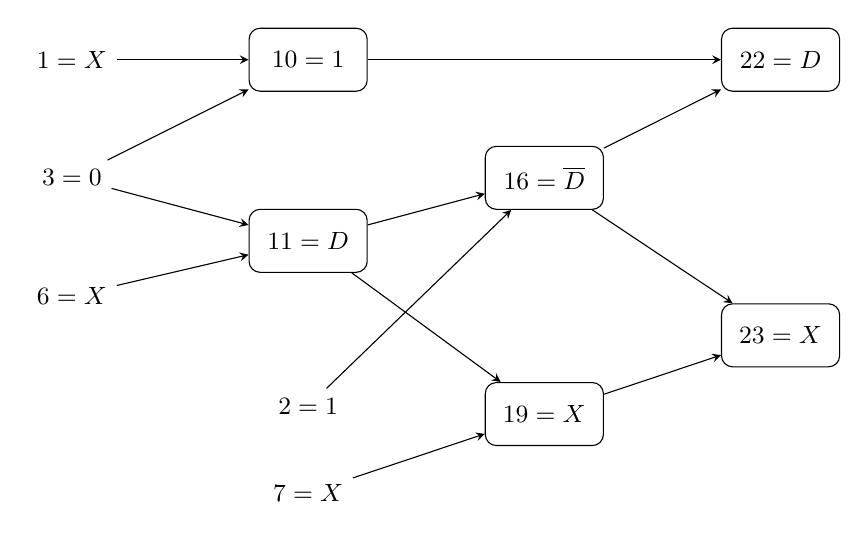
\begin{tikzpicture}[x=1cm,y=1cm,every node/.style={font=\small},gate/.style={draw,rounded corners,minimum width=1.5cm,minimum height=0.8cm,align=center},>=stealth]
\node (i1) at (0,3) {$1=X$}; \node (i3) at (0,1.5) {$3=0$};
\node (i6) at (0,0) {$6=X$}; \node (i2) at (3,-1.4) {$2=1$};
\node (i7) at (3,-2.5) {$7=X$};
\node[gate] (g10) at (3,3) {$10=1$};
\node[gate] (g11) at (3,0.7) {$11=D$};
\node[gate] (g16) at (6,1.5) {$16=\overline D$};
\node[gate] (g19) at (6,-1.5) {$19=X$};
\node[gate] (g22) at (9,3) {$22=D$};
\node[gate] (g23) at (9,-0.5) {$23=X$};
\draw[->] (i1)--(g10); \draw[->] (i3)--(g10); \draw[->] (i3)--(g11); \draw[->] (i6)--(g11);
\draw[->] (g11)--(g16);\draw[->] (g11)--(g19);\draw[->] (i2)--(g16);\draw[->] (i7)--(g19);
\draw[->] (g10)--(g22);\draw[->] (g16)--(g22);\draw[->] (g16)--(g23);\draw[->] (g19)--(g23);
\end{tikzpicture}
